\subsection{Simplified template cross section}
\label{subsec:stxs}

The measurements of the product $\sigma\cdot\mathcal{B}$ of the Higgs boson production cross-section and the branching ratio normalised by the SM expectation,
$(\sigma\cdot\mathcal{B})_{\mathrm{SM}}$, for the stages of production bins defined in Section~\ref{subsec:STXS_Categories} are shown in Fig.~\ref{fig:stxs_0} for the stage 0 and in Fig.~\ref{fig:stxs_1} for the reduce stage 1.2.
The corresponding numerical values are given in Table~\ref{tab:stage0} and Table~\ref{tab:stage1p2}.
In the ratio calculation, the uncertainties in the SM expectation are not taken into account while the theoretical uncertainties which can cause migration of events between the various categories are kept in this measurement.
The correlation matrices are shown in Fig.~\ref{fig:corrmatrix}.
The dominant experimental sources of systematic uncertainty are the same as in the measurement of the signal-strength modifiers, while the dominant theoretical source is the uncertainty in the category migration for the $\ggH$ process.

As for the signal strenght, all measurements are reported at $\mH=125.38$ GeV.%, the best mass obtained by CMS from the combination of $H\rightarrow$ZZ and $H\rightarrow\gamma\gamma$ channels.

%%%%%%%%%%%%%%%%%%%%%%%
\begin{figure}[!htb]
\begin{center}
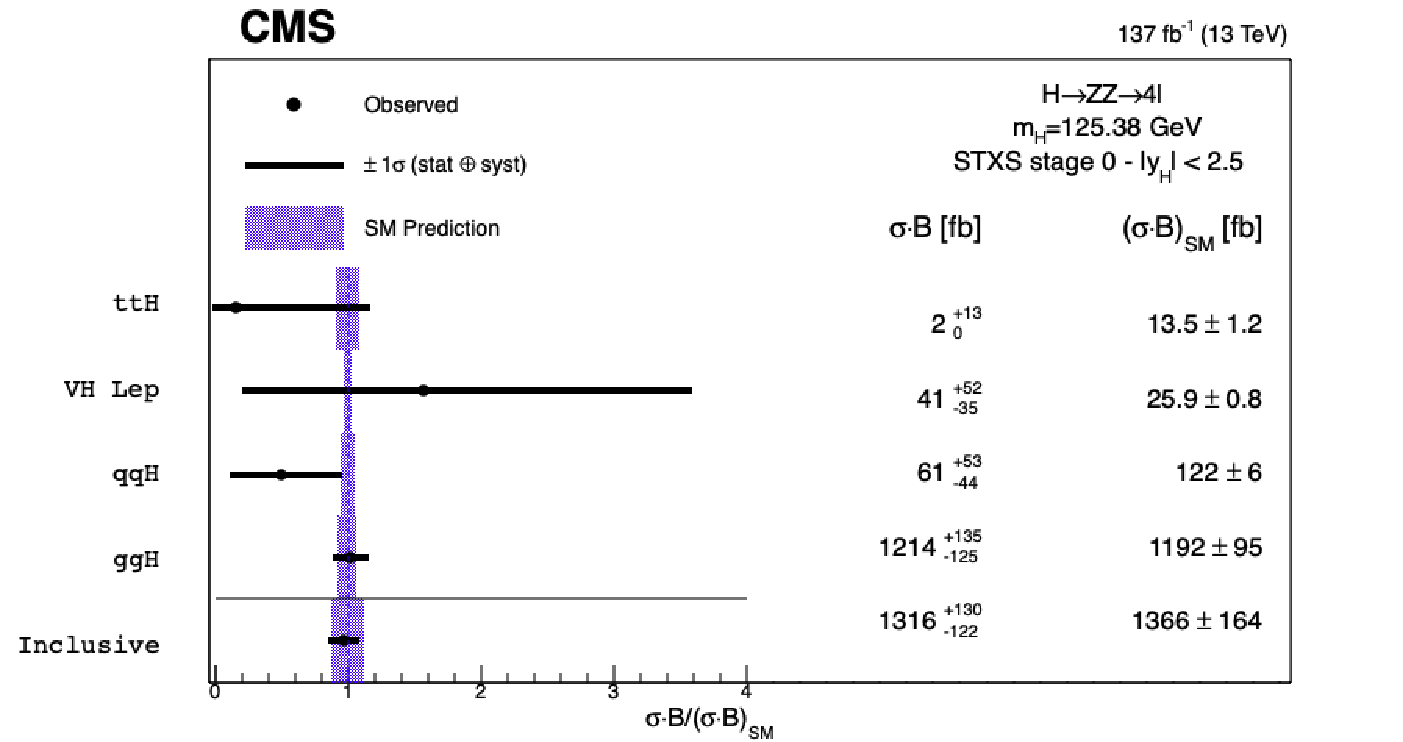
\includegraphics[width=0.7\linewidth]{Figures/results/stxs/stage0_125_38.pdf}
\caption{
		The ratios between measured cross sections $\sigma\cdot\mathcal{B}$ and the SM predictions $(\sigma\cdot\mathcal{B})_{\mathrm{SM}}$ for the stage 0 production bins.%, with $\mH$ profiled in the fit.
		The gray band around the vertical band shows the theoretical uncertainties on the SM Higgs boson cross section predictions for each of the bin.
		%Cross section values are reported for the best fit mass value $\mH = 125.1~\GeV$.
			\label{fig:stxs_0}
			}
	\end{center}
\end{figure}
%%%%%%%%%%%%%%%%%%%%%%%

%%%%%%%%%%%%%%%%%%%%%%%
\begin{table}[hb]
	\begin{center}
		\caption{
		Best-fit values and $\pm 1\sigma$ uncertainties for the measured cross sections $\sigma\cdot\mathcal{B}$ and the SM predictions $(\sigma\cdot\mathcal{B})_{\mathrm{SM}}$ for the stage 0 production bins.
		The results are obtained with $\mH=125.38$ GeV. % profiled in the fit.
		\label{tab:stage0}
			}
    \renewcommand{\arraystretch}{1.5}
    \begin{tabular}{ccc}
	\hline
	& $\sigma\cdot\mathcal{B}$ & $(\sigma\cdot\mathcal{B})_{\mathrm{SM}}$ \\
	\hline
        {\tt ttH} & $2~^{+13}_{-2}~$fb & $13~^{+18}_{-10}~$fb \\
	{\tt VH-lep} & $41~^{+52}_{-35}~$fb & $26~^{+42}_{-25}~$fb \\
	{\tt qqH} & $61~^{+53}_{-44}~$fb & $122~^{+62}_{-52}~$fb \\
%	{\tt ggH} & $1214~\pm 124~$fb & $1174\pm 123~$fb \\
	{\tt ggH} & $1214~^{+135}_{-125}~$fb & $1192~^{+139}_{-129}~$fb \\
    \hline
    {\tt Inclusive} & $1316~^{+130}_{-122}~$fb & $1366~^{+138}_{-126}~$fb  \\
	\hline
	\end{tabular}
 \end{center}
 \end{table}
 %%%%%%%%%%%%%%%%%%%%%%%

%%%%%%%%%%%%%%%%%%%%%%%
\begin{figure}[!htb]
\begin{center}
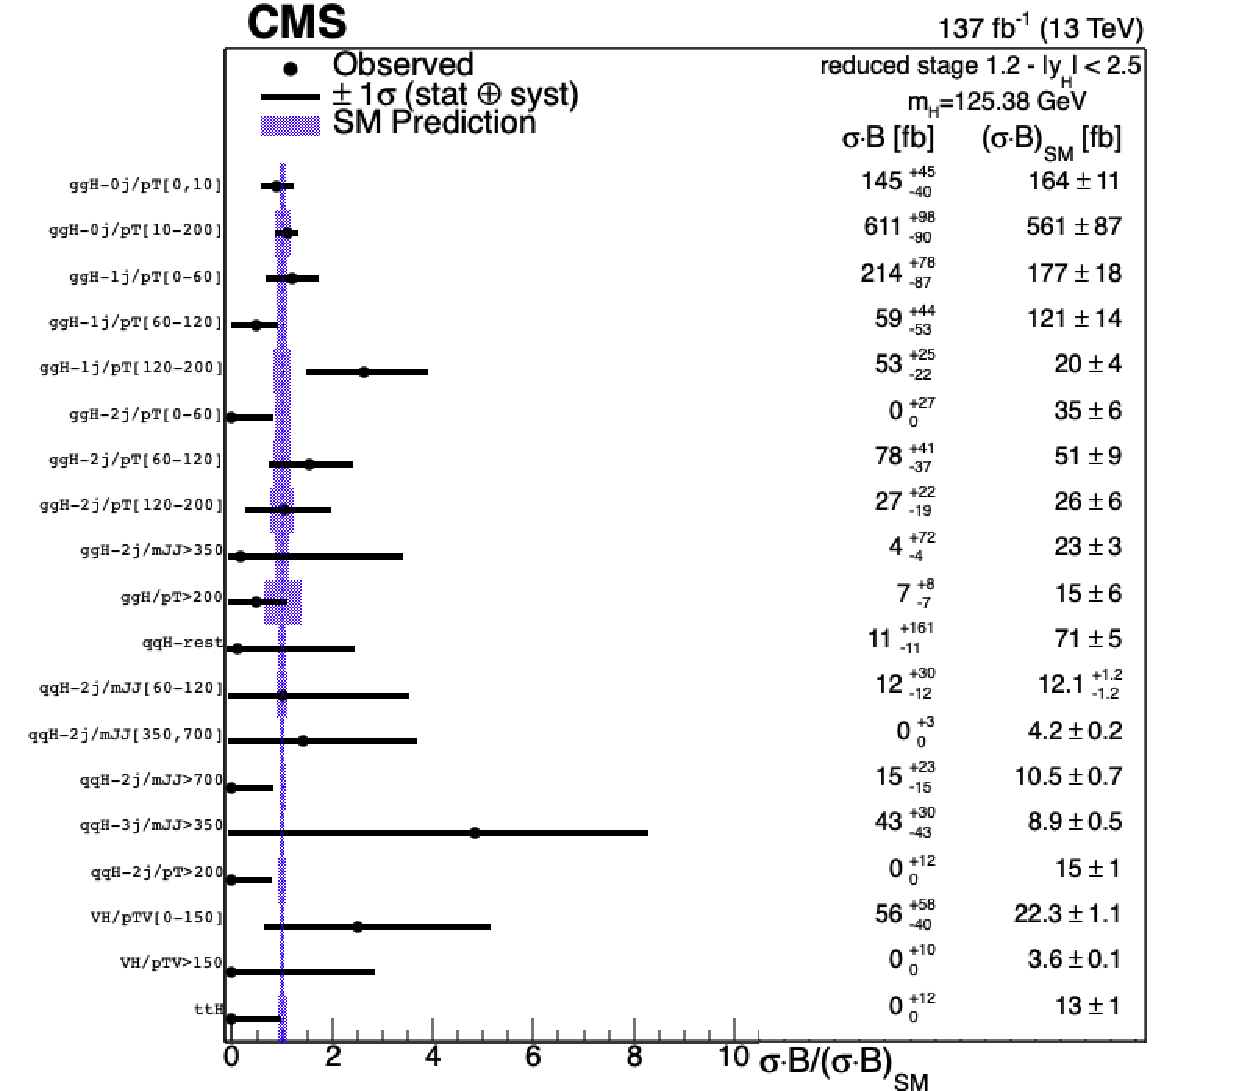
\includegraphics[width=0.9\linewidth]{Figures/results/stxs/stage1p2_125_38.pdf}
\caption{
The ratios between measured cross sections $\sigma\cdot\mathcal{B}$ and the SM predictions $(\sigma\cdot\mathcal{B})_{\mathrm{SM}}$ for the merged stage 1.2 production bins, with $\mH=125.38$ GeV. % profiled in the fit.
The gray band around the vertical band shows the theoretical uncertainties on the SM Higgs boson cross section predictions for each of the bin.
\label{fig:stxs_1}
}
\end{center}
\end{figure}
%%%%%%%%%%%%%%%%%%%%%%%

%%%%%%%%%%%%%%%%%%%%%%%
\begin{table}[hb]
	\begin{center}
		\caption{
		Best-fit values and $\pm 1\sigma$ uncertainties for the measured cross sections $\sigma\cdot\mathcal{B}$ and the SM predictions $(\sigma\cdot\mathcal{B})_{\mathrm{SM}}$ for the stage 1.2 production bins.
		The results are obtained with $\mH$ profiled in the fit.
		\label{tab:stage1p2}
			}
    \renewcommand{\arraystretch}{1.5}
    \begin{tabular}{ccc}
	\hline
	& $\sigma\cdot\mathcal{B}$ & $(\sigma\cdot\mathcal{B})_{\mathrm{SM}}$ \\
	\hline
	{\tt ggH-0j/pT[0-10]} & $145~^{+45}_{-40}~$fb & $164~^{+48}_{-42}~$fb \\
	{\tt ggH-0j/pT[10-200]} & $611~^{+98}_{-90}~$fb & $560~^{+98}_{-91}~$fb \\
	{\tt ggH-1j/pT[0-60]} & $214~^{+78}_{-87}~$fb & $177~^{+98}_{-91}~$fb \\
    {\tt ggH-1j/pT[60-120]} & $59~^{+44}_{-53}~$fb & $121~^{+66}_{-55}~$fb \\
	{\tt ggH-1j/pT[120-200]} & $53~^{+25}_{-22}~$fb & $20~^{+21}_{-18}~$fb \\
	{\tt ggH-2j/pT[0-60]} & $0~^{+27}_{-0}~$fb & $35~^{+53}_{-35}~$fb \\
	{\tt ggH-2j/pT[60-120]} & $78~^{+41}_{-37}~$fb & $51~^{+50}_{-42}~$fb \\
	{\tt ggH-2j/pT[120-200]} & $27~^{+22}_{-19}~$fb & $26~^{+27}_{-21}~$fb \\
	{\tt ggH-2j/mJJ>350} & $4~^{+72}_{-4}~$fb & $23~^{+57}_{-0.23}~$fb \\
	{\tt ggH/pT>200} & $7~^{+8}_{-7}~$fb & $15~^{+15}_{-12}~$fb \\
	{\tt qqH-rest} & $11~^{+161}_{-11}~$fb & $71~^{+190}_{-71}~$fb \\
	{\tt qqH-2j/mJJ[60-120]} & $12~^{+30}_{-12}~$fb & $12~^{+69}_{-12}~$fb \\
	{\tt qqH-2j/mJJ[350-700]} & $0~^{+3}_{-0}~$fb & $4~^{+9}_{-4}~$fb \\
	{\tt qqH-2j/mJJ>700} & $15~^{+23}_{-15}~$fb & $10~^{+26}_{-10}~$fb \\
	{\tt qqH-3j/mJJ>350} & $43~^{+30}_{-43}~$fb & $9~^{+35}_{-9}~$fb \\
	{\tt qqH-2j/pT>200} & $0~^{+12}_{-0}~$fb & $15~^{+20}_{-14}~$fb \\
	{\tt VH-lep/pTV[0-150]} & $56~^{+58}_{-40}~$fb & $22~^{+44}_{-22}~$fb \\
	{\tt VH-lep/pTV>150} & $0~^{+10}_{-0}~$fb & $4~^{+16}_{-4}~$fb \\
	{\tt ttH} & $0~^{+12}_{-0}~$fb & $13~^{+18}_{-10}~$fb \\
	\hline
	\end{tabular}
 \end{center}
 \end{table}
 %%%%%%%%%%%%%%%%%%%%%%%

%%%%%%%%%%%%%%%%%%%%%%%
\begin{figure}[!htb]
	\begin{center}
		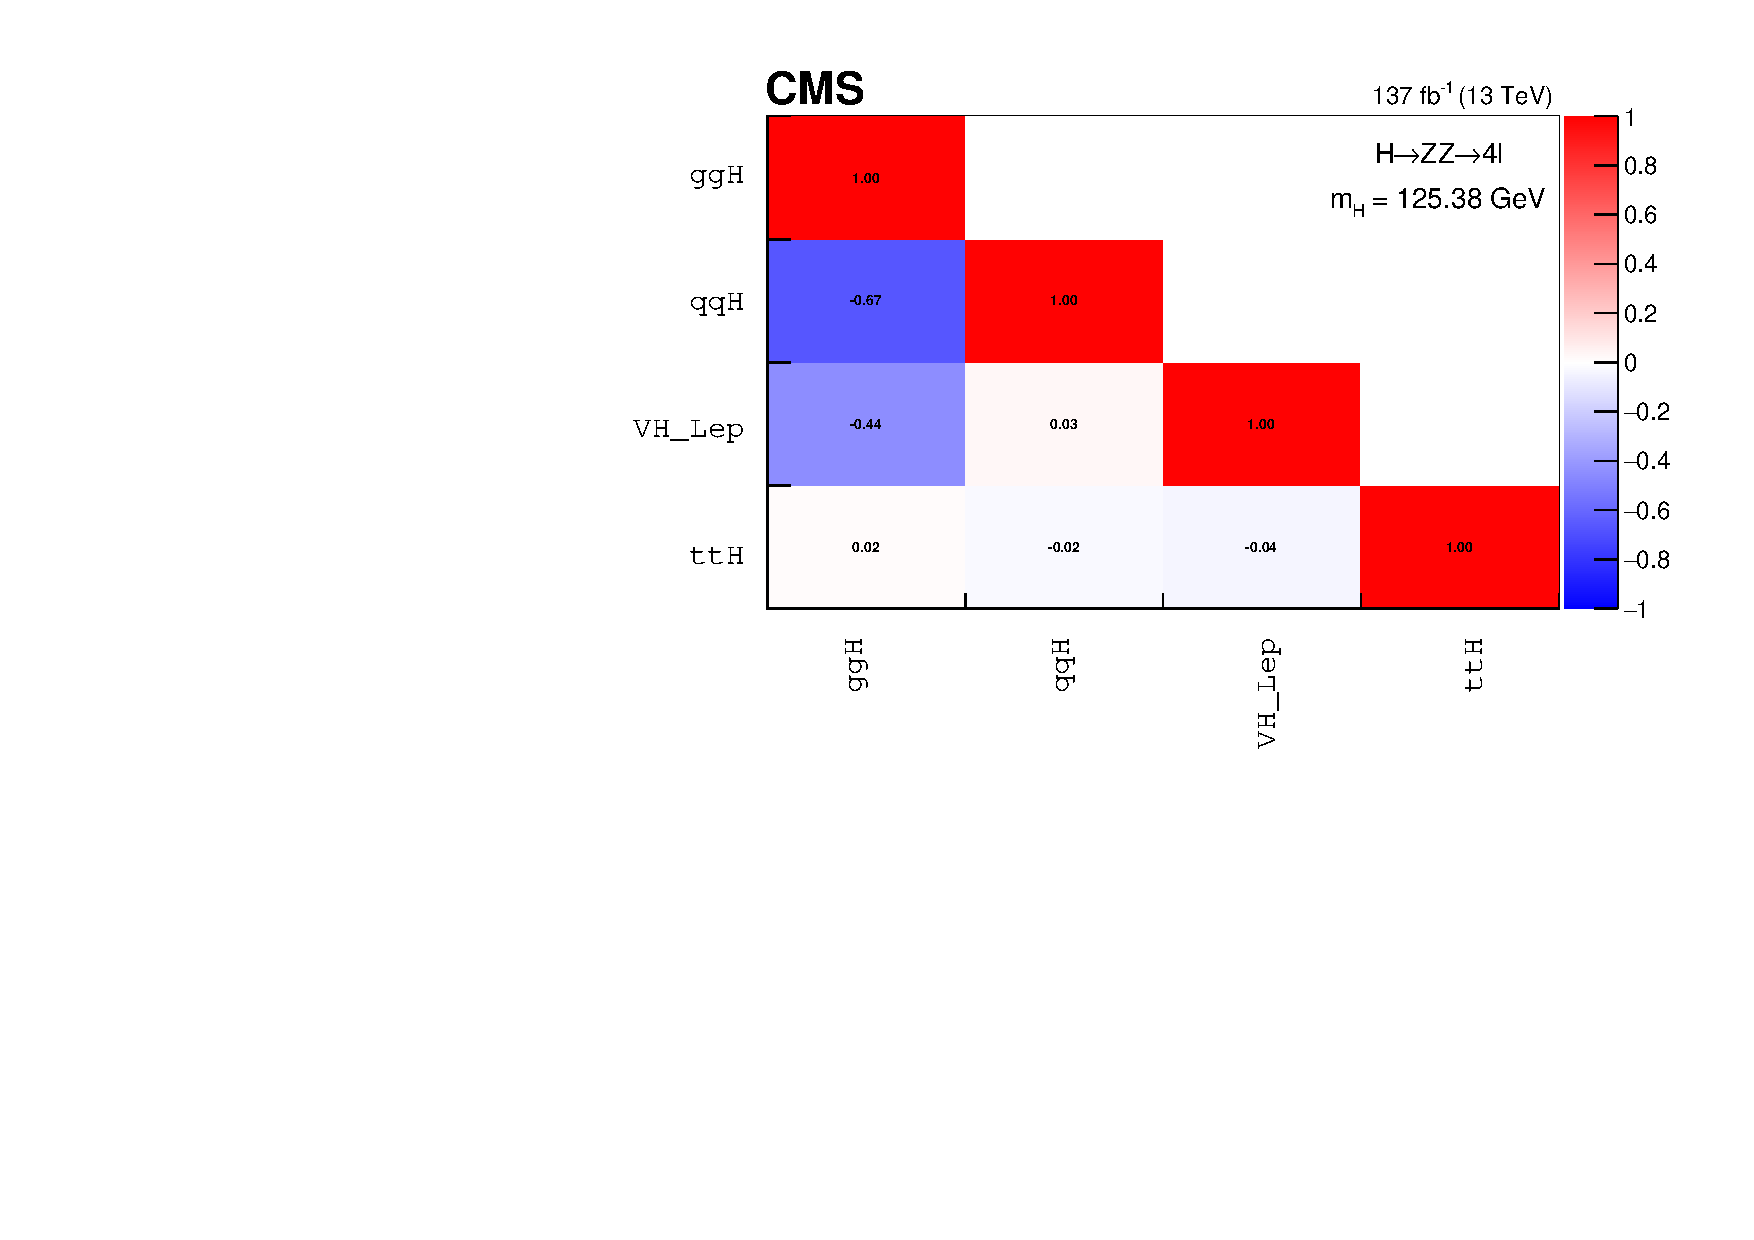
\includegraphics[height=0.6\linewidth]{Figures/results/stxs/scov_stxs0_125_38.pdf}
		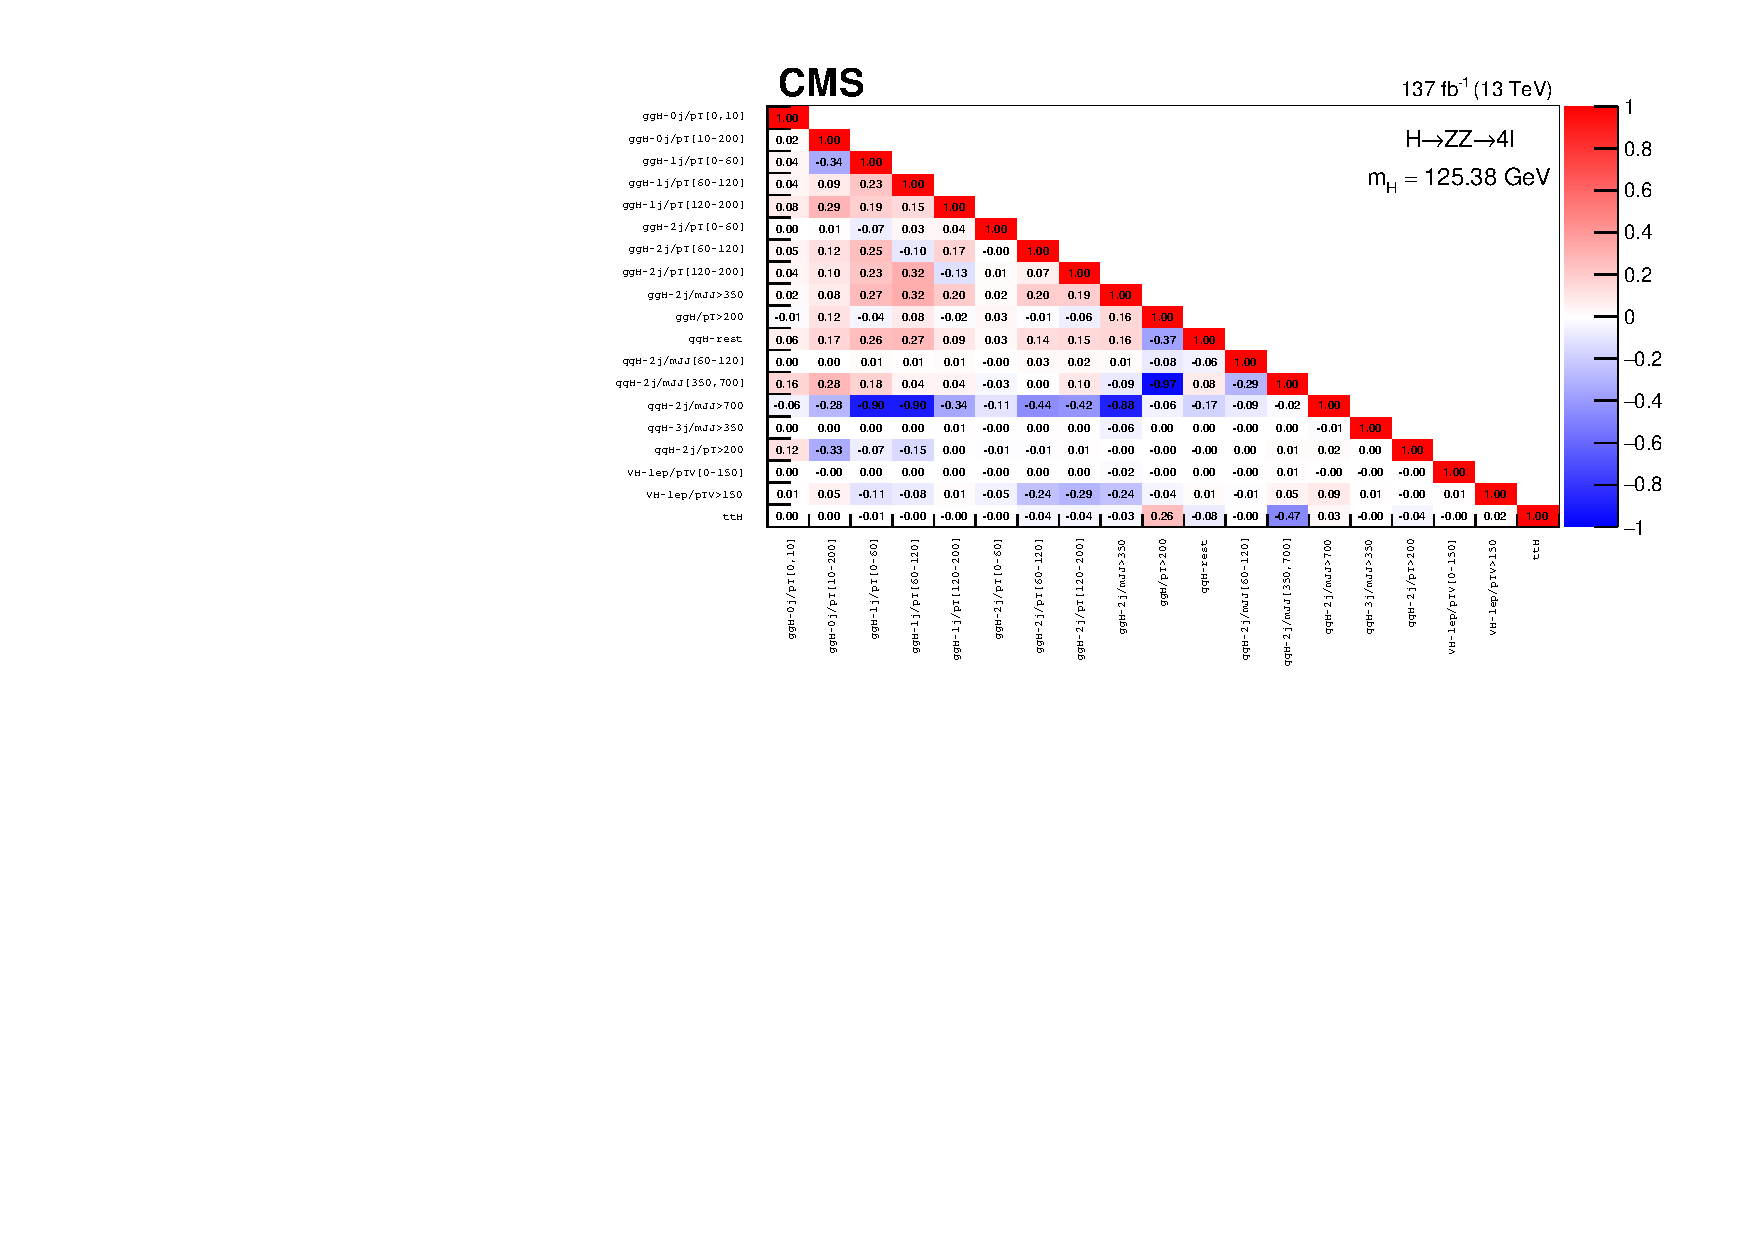
\includegraphics[height=0.6\linewidth]{Figures/results/stxs/scov_stxs1p2_125_38.pdf}
		\caption{The correlation matrices between the measured cross-sections are shown for the stage 0 (left) and the merged stage 1.2 (right).
			\label{fig:corrmatrix}}
	\end{center}
\end{figure}
%%%%%%%%%%%%%%%%%%%%%%%




%In this section we present the results for simplified template cross sections Stage 1.1, a measurement strategy detailed in the CERN Yellow Report 4 of the LHC-HXSWG~\cite{YR4}. The reduced stage 1.1 bins are measured in forms of signal strength modifier. Figure~\ref{fig:stage1p1_mu} shows the results. The covariance matrix of the fitted results are shown in Figure~\ref{fig:cov} 

%%=======
%\begin{figure}[!htb]
%        \vspace*{0.3cm}
%        \begin{center}
%                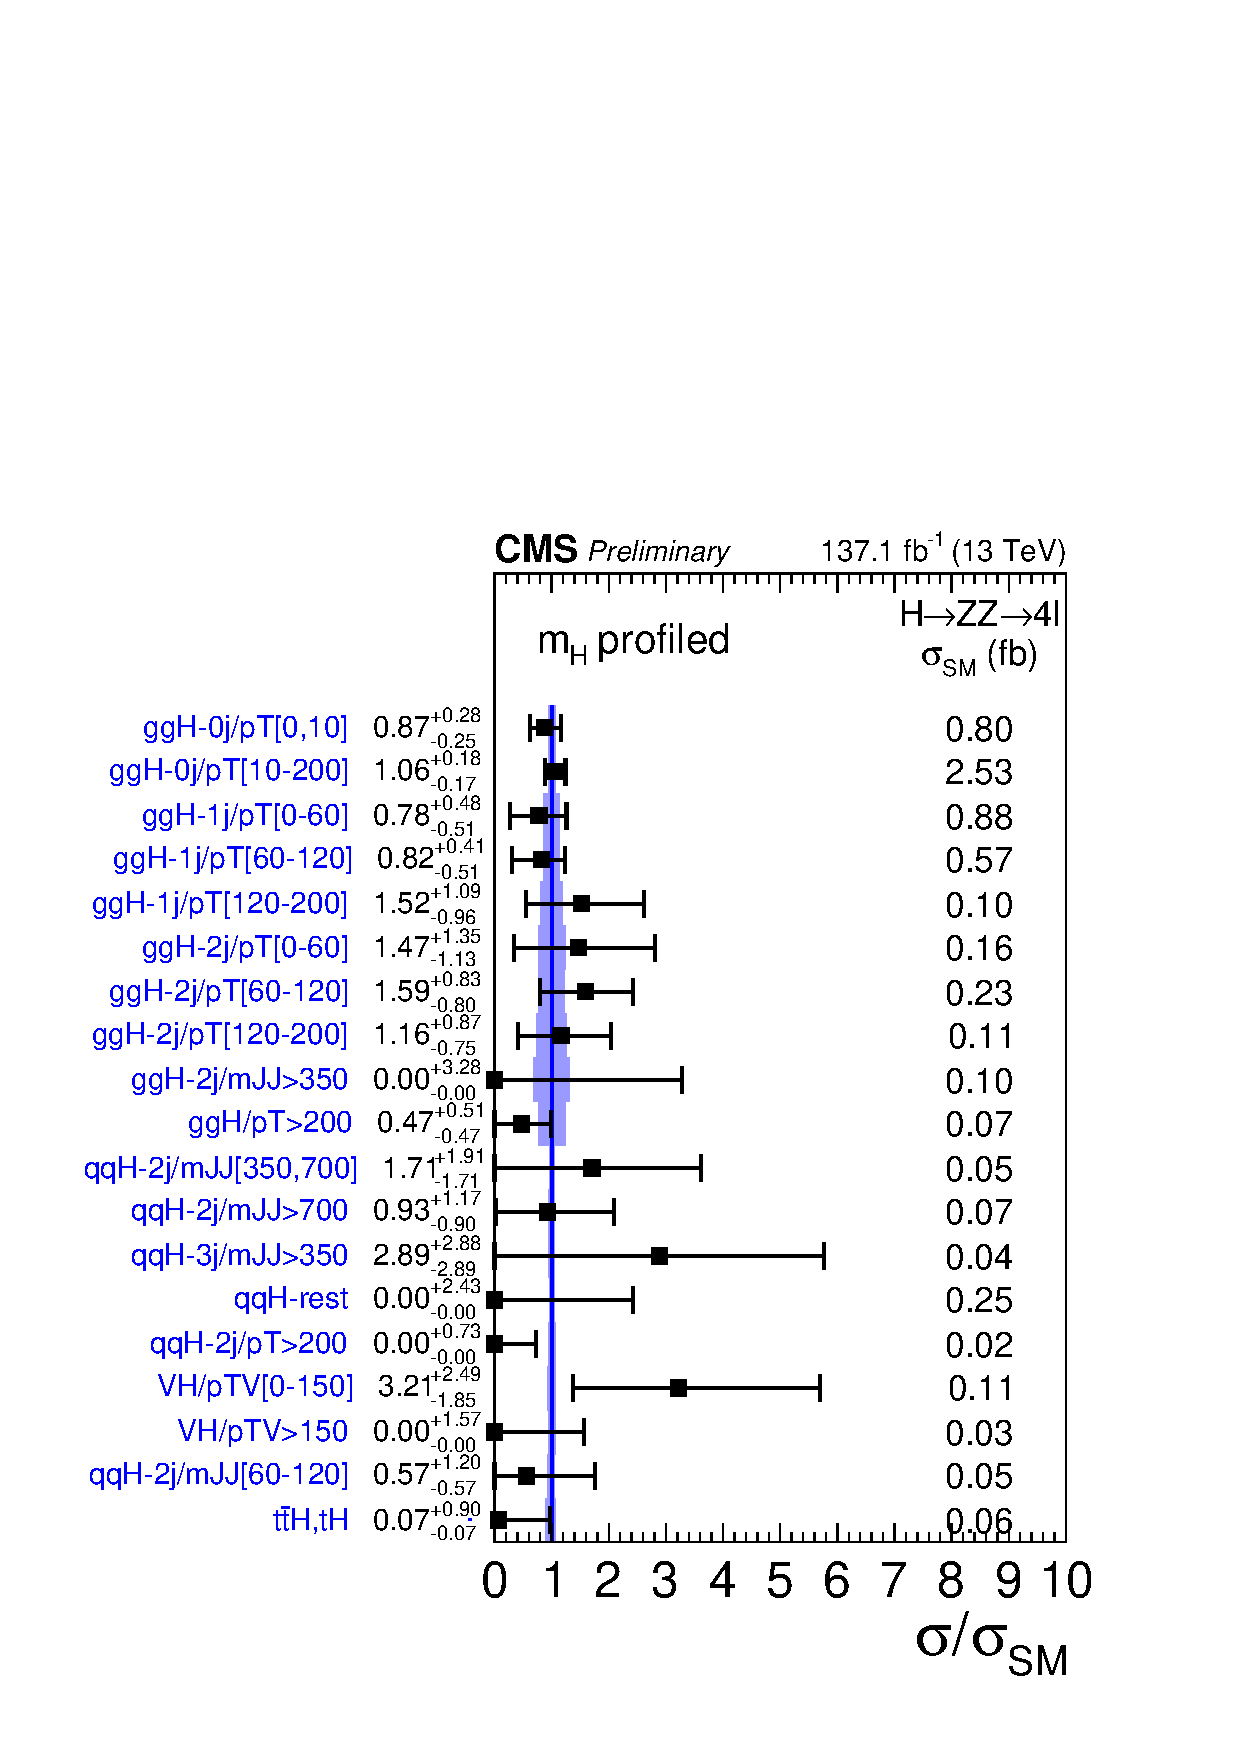
\includegraphics[width=0.8\textwidth]{Figures/results/stxs/mu_stage1_xsec.pdf}
%                \caption{The ratios between measured cross sections and the SM prediction for stage1.1 bins, the \mH is profiled. The band around the vertical band shows the theoretical uncertainties on the SM cross section predictions for each stage 1.1 bin.}
%                \label{fig:stage1p1_mu}}
%        \end{center}
%\end{figure}
%=======

%=======
%\begin{figure}[!htb]
%        \vspace*{0.3cm}
%        \begin{center}
%                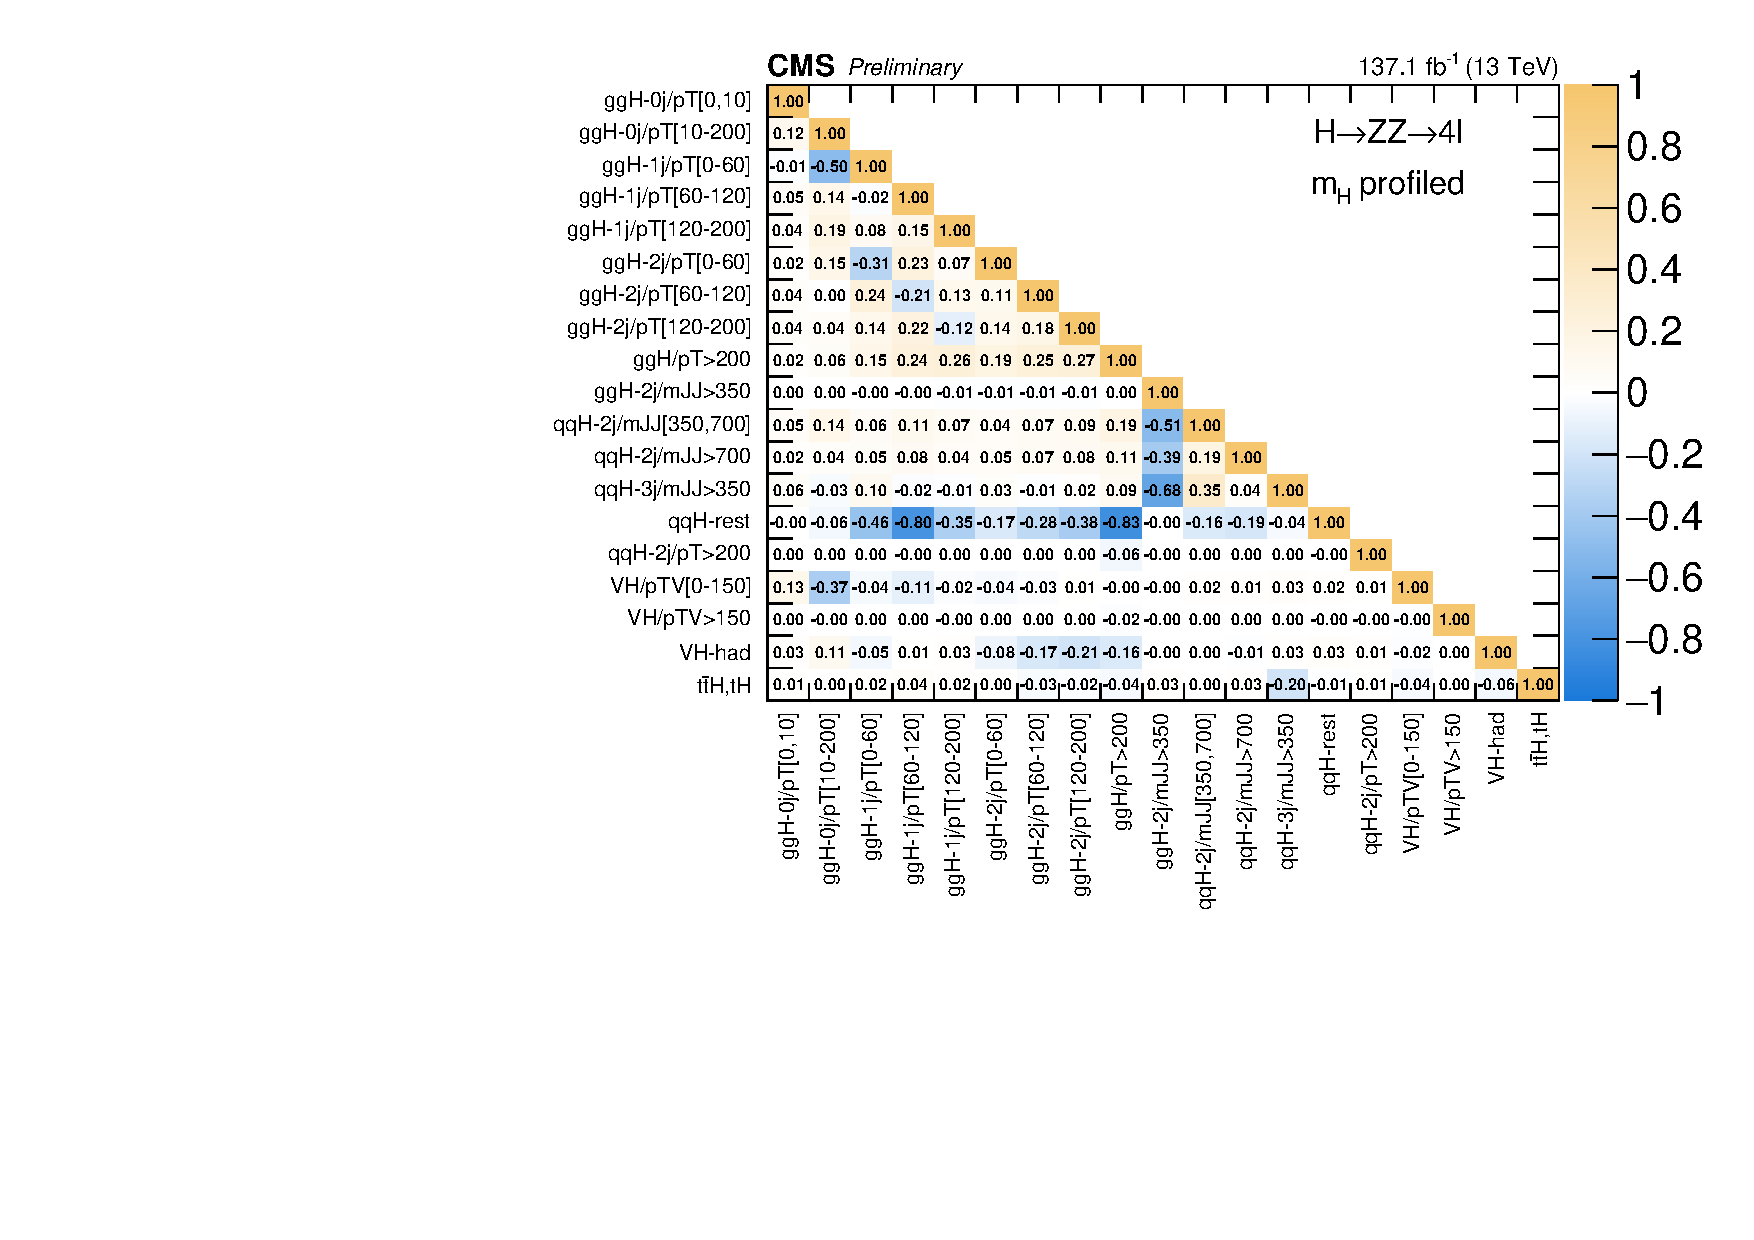
\includegraphics[width=0.8\textwidth]{Figures/results/stxs/scov_stage1.pdf}
%                \caption{Covariance matrix of the fitted signal strength.}
%                \label{fig:cov}}
%        \end{center}
%\end{figure}
%=======
